\begin{frame}{Dise�o del Sistema HAR}

\framesubtitle{Metodolog�a y Sistemas HAR}

\setbeamercovered{transparent}
\begin{spacing}{0}
\begin{center}
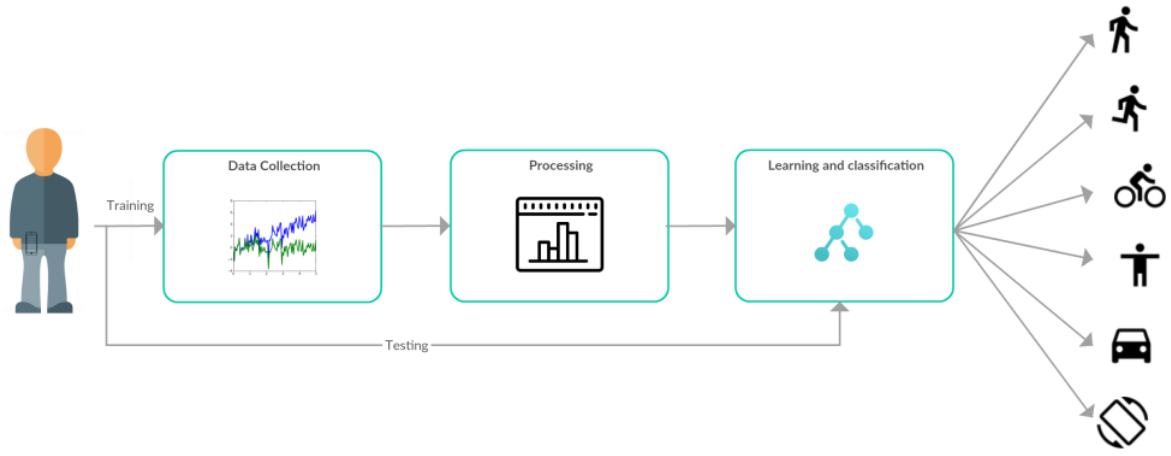
\includegraphics[width=0.85\textwidth]{../capitulo-2/graphics/harsystem2}
\par\end{center}
\end{spacing}
\begin{columns}[t]

\column{0.5\textwidth}
\begin{itemize}
\item Componentes principales
\begin{itemize}
\item un \structure{recolector} de medidas 
\item un \structure{procesador} de muestras 
\item un \structure{clasificador} de actividades
\end{itemize}
\end{itemize}

\pause{}

\column{0.5\textwidth}
\begin{itemize}
\item Metodolog�a operativa
\begin{itemize}
\item Aprendizaje fuera de linea (\emph{off-line})
\item Clasificaci�n en linea (\emph{on-line})
\end{itemize}
\end{itemize}
\end{columns}

\end{frame}
%

